\epigraph{``The grandest discoveries of science have been but the rewards of
    accurate measurement and patient long-continued labour in the minute
sifting of numerical results.''}{William Thompson, \nth{1} Baron Kelvin}

\section{Models of the Atomic Nucleus}

To unravel the nuclear many-body problem, we can
employ models that incorporate essential details while ignoring specifics with
little relevance to the observables we care about.

Successful models possess both accuracy at reproducing extant experimental data
and predictive power for as-yet unmeasured experimental data (far harder). For parametric models
with many tunable parameters, these criteria pull in oppositive directions: increasing the number
and acceptable range of model parameters often helps to reproduce experimental data but may
jeopardize predictive power if new parameters are not connected to the underlying physics.

\subsection{Liquid Drop Model}

An especially simple and
effective model, the Liquid Drop Model (LDM), describes nuclei as drops of
an ideal nuclear fluid and has been successfully employed for many decades to
describe nuclear masses. The binding forces of each nucleus are modeled by five
physically-intuitive terms appropriate for such a fluid:

a volume term that describes "bulk" binding that would be experienced in an
infinite sea of nuclear matter, or  by completely surrounded nucleons in the core of the nucleus,

a surface term that incorporates the finite size of a nucleus (i.e., it is a
drop, not an ocean), equivalent to surface tension,

a coulomb term that incorporates the electric repulsion experienced by protons
constrained in close proximity to each other inside the drop,

an asymmetry term representing the relative chemical potential of neutrons and
protons as a function of their relative population (which can be re-balanced by
beta-decay),

and a spin-orbit term responsible for modeling the interaction of the intrinsic spin
of a nucleus and its constituent nucleons' angular orbital momentum, which is
a much stronger effect in nuclear binding than in the atomic case

In this model, each term is parameterized and the ensemble can be fitted to
well-measured nuclear masses across the chart of nuclides. Happily, though the detailed
quantum structure is completely ignored, these five terms are quite successful
in describing nuclear masses.

\cite{MyersAndSwiatecki}

In the droplet model, the symmetry energy $J$, density dependence of the symmetry energy
$L$, and surface stiffness coefficient $Q$ are the primary variables determining the formation of a 
neutron skin \ref{Myers1980}.

\subsection{Mean Field Models}

Independent Particle Model (IPM)
HF
BHF
RPA

The Independent Particle Model (IPM) provides a complementary approach expressly
focused on the quantum details of the problem. The many-body problem is
approximated by considering each nucleon as moving independently of all other
nucleons in an potential generated by those nucleons. As in the atomic case,
where electrons obey an aufbau principle and populate orbitals defined by the
atomic potential, both protons and neutrons obey a nuclear aufbau, filling
orthogonal states in the nuclear potential. In this model, many fundamental
quantum properties of nuclei are easily understood, (for example, ground state spins and
the appearance of shell closures in direct analogy to the atomic case).
Unfortunately, the assumption of independent nucleon motion that defines the model
also kneecaps its usefulness: in reality, nuclear systems are strongly
correlated and exhibit clustering and collective motion, behaviors at odds with the
the IPM picture.

\subsection{Effective Field Theories}
Connect to chiral effective field theory work for calculating optical potentials
and examining isovector component of potential, especially w/r/t to exotic
nuclei near driplines.

\subsection{Density Functional Theory}
Fission
Heavy systems (no lighter than Ca40)

\subsection{Optical Models}
Hodgson's optical model review in 1971

- Microscopic (folds interaction over nucleon density)
- Phenomenological (no folding - use bulk)

Optical Model description of the nucleus
-> can largely follow Bob and Wim's review paper
- first formulated in 1949 to describe neutron cross section data
- separate proton and neutron global optical potentials in the 60s (Becchetti
and Greenlees)
- CH89 includes additional neutron scattering data on isotopic targets

Takeaway: neutron scattering data particularly valuable for constraining these
models, but particularly challenging to access experimentally.

"The magnitude and energy dependence of the real isovector part of the
optical potential are poorly constrained by experiment." \cite{Holt16}

Lane potential 

Isovector versus isoscalar. Charged pion exchange mediates the isovector forces;
other nucleon-nucleon interactions mediate the isoscalar forces.

The Dispersive Optical Model, the model used in this thesis to analyze experimental scattering data
and extract structural information, is the subject of Chapter \ref{DOMFormalism}, where a brief
formal treatment is given.

Connect to Vinas, Chuck Horowitz, and J. Piekarewicz's neutron star EOS work.

Connect to FRIB/study of extremely neutron-rich systems relevant for r-process
and astrophysical nucleosynthesis.

\section{Nuclear Experimental Data}
\subsection{Elastic nucleon scattering}
\subsection{Inelastic nucleon scattering}

New neutron scattering data (both \tot and \el) on isotopic targets, grist for the DOM mill and the 
central result of this dissertation, are presented in Chapters \ref{TCSAnalysis, ECSAnalysis}.

Neutron scattering is a direct, Coulomb-insensitive tool for probing the nuclear
environment. The simplest measurement of neutron interaction with a nucleus,
the neutron total cross section \totE, provides fundamental information about
nuclear size and the ratio of elastic-to-inelastic components of nucleon 
scattering. Additionally, \tots data are sensitive to a variey of nuclear
properties of great interest including the neutron skin of neutron-rich nuclei
\cite{Mahzoon2017} and thus the density dependence of the symmetry energy $L$,
essential for an accurate neutron star equation-of-state (EOS)
\cite{Fattoyev2012, Vinas2014, Brown2000}.

The earliest model for neutron scattering (a ``strongly-absorbing sphere"
picture) describes the nucleus as a constant-density sphere that interacts
strongly with incident neutrons approaching within a nuclear radius
\cite{Feshbach1949}. In this picture devoid of nuclear structure, \totEs depends
only on size scaling of the interacting bodies:
\begin{equation} \label{SASAbsolute}
    \sigma_{tot}(E) = 2\pi(R + \lambdabar)^{2}
\end{equation}
where $R=r_{0}A^{\frac{1}{3}}$ and $\lambdabar$ is the reduced wavelength
of the incident neutron in the center of mass \cite{Fernbach1949, Satchler1980}. 
To compare \totEs for two different targets of masses A and A', the relative
difference \totRDs is useful:
\begin{equation} \label{SASRelDiff}
    \begin{split}
        \totRDs & \equiv
    \frac{\sigma_{A}-\sigma_{A'}}{\sigma_{A}+\sigma_{A'}} \\
    & =
    \frac{r_{0}^{2}(A^{\frac{2}{3}}-A'^{\frac{2}{3}}) +
    2\lambdabar r_{0}(A^{\frac{1}{3}}-A'^{\frac{1}{3}})}
    {r_{0}^{2}(A^{\frac{2}{3}}+A'^{\frac{2}{3}}) +
    2\lambdabar r_{0}(A^{\frac{1}{3}}+A'^{\frac{1}{3}}) + 2\lambdabar^{2}}
    \end{split}
\end{equation}
While on \textit{average}, experimental data comport with this naive
model, the key feature of \totEs data is the obvious oscillatory
behavior centered about the average (visible in Fig.
\ref{SASphereVsExperiment}).

\begin{figure*}
    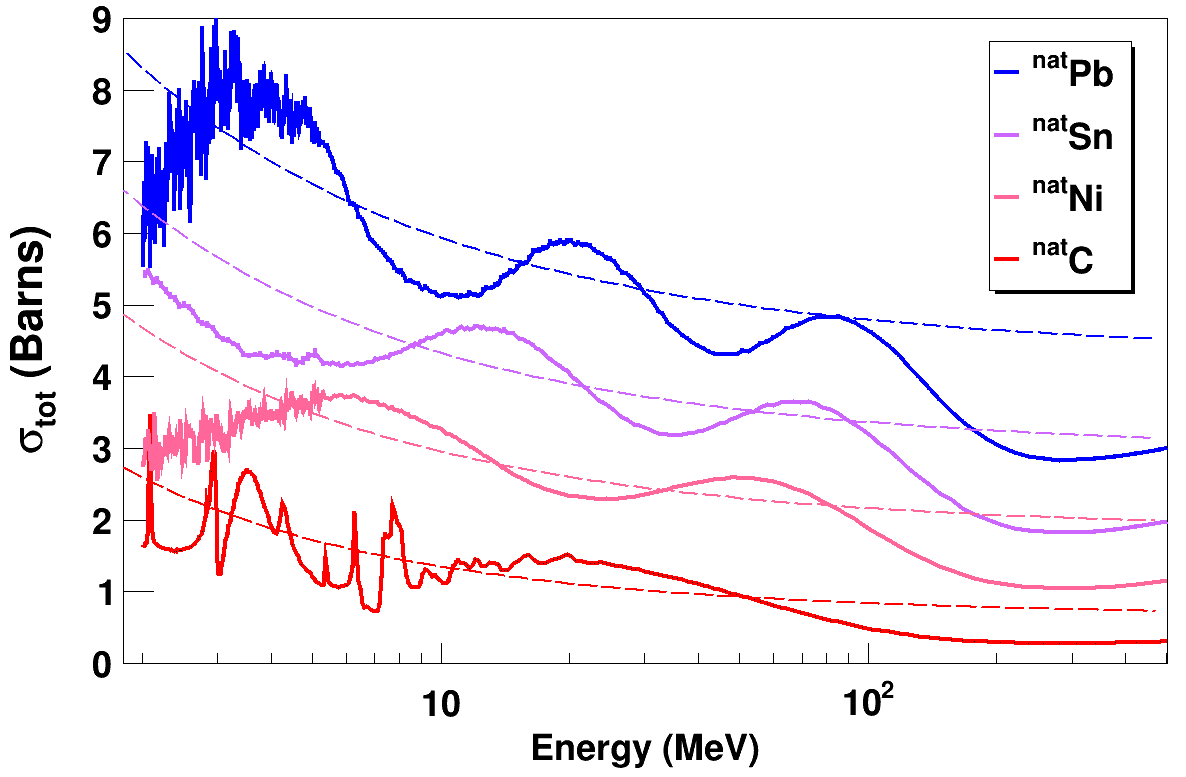
\includegraphics[scale=0.3]{../analysis/plots/theory/SASphereVsExperiment.png}
    \caption{Experimental neutron \tot\ data and strongly-absorbing-sphere predictions for \cNat, \niNat, \snNat, \pbNat}
    \label{SASphereVsExperiment}
\end{figure*}

Experimental \totEs data are shown from 2-500
MeV for nuclides from A=12 to A=208
\cite{Finlay1993, Schwartz1974, Poenitz1983, Abfalterer2000, Abfalterer2001}.
Predictions for \totEs given by the ``strongly-absorbing sphere" (SAS)
model, Eq. \ref{SASAbsolute}, are shown as thin dashed lines for each nucleus.
Regular oscillations about the SAS model are clearly visible
as is the trend for the oscillation
maxima/minima to shift to \textit{higher} energies as A is increased. At low energies 
resonance structures are visible especially for light nuclides where the
density of states is smallest. Note that at higher energies, the experimental
cross sections drop below those predicted by the SAS model, illustrating
the failure of the SAS model to describe [surface physics accounted for in
optical models?].

These oscillations can be explained as the result of a phase shift between 
neutron waves passing around the nucleus (unshifted) and waves passing
through the the nucleus, where they experience refraction
(illustrated in Fig. \ref{RamsauerPhaseShiftFigure}). This explanation was termed the ``nuclear 
Ramsauer effect" by Peterson \cite{Peterson1962}, based on the analagous effect seen in 
electron scattering on noble gases.
In this picture, the intractable many-body
problem of the target nucleus is replaced by a smooth potential (hence the
``optical model" of the nucleus, \cite{Feshbach1958}) from which the refractive
index is easily calculated. As in the optical case, a complex index of
refraction can be used to neatly incorporate both elastic scattering (the real
potential) and all other scattering removing flux from the elastic channel (the imaginary potential).
%\cite{McVoy1967}. 

\begin{figure}
    \hfill\begin{minipage}{0.5\textwidth}\centering
        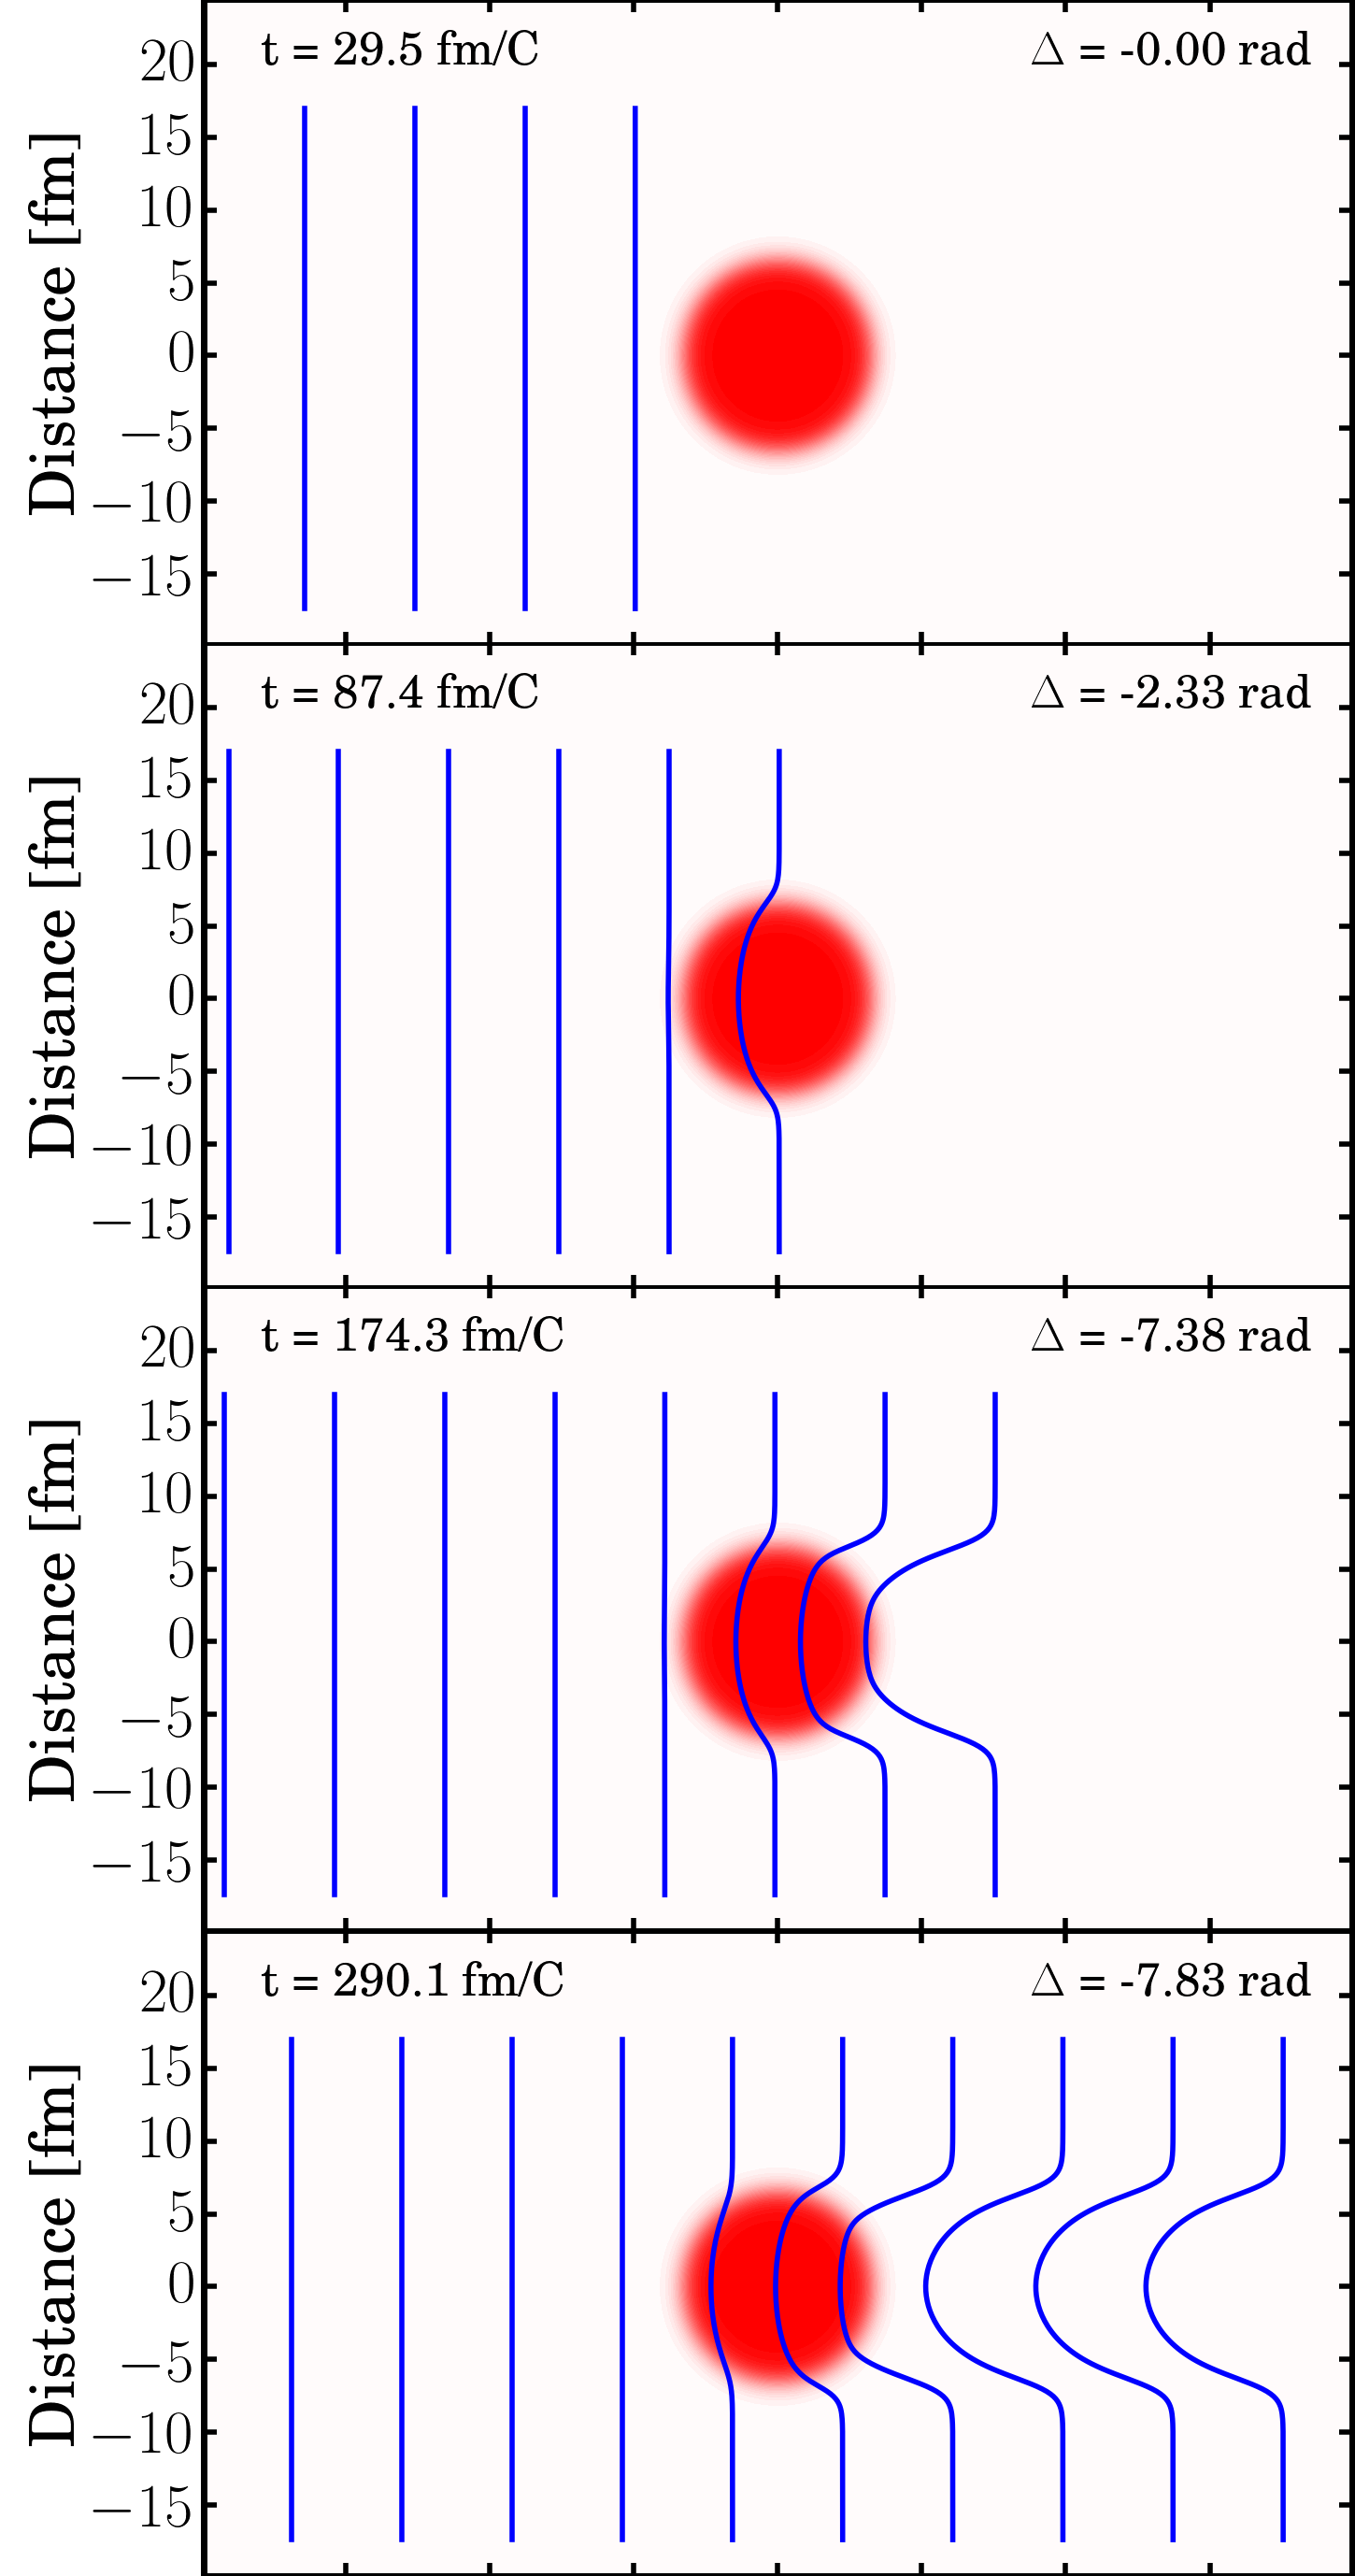
\includegraphics[scale=0.2]{figures/phaseShiftStillsFigure.png}
        \caption{A simplified illustration of the nuclear Ramsauer effect}
        \label{RamsauerPhaseShiftFigure}
    \end{minipage}
\end{figure}

 A neutron wave train (series of
            blue lines) impinges from the left on a real Woods-Saxon
            potential centered at the origin (diffuse red circle). The potential
            refracts the neutron wave,
            retarding the phase of the wavefront as it passes through the
            potential. After escaping the potential, a phase difference $\Delta$ between
            the wave component passing \textit{around} and \textit{through the center}
            of the potential persists, resulting in scattering.
            For the leading wavefront in the wave train, $\Delta$ is indicated in
            the top right-hand corner of each panel. A differential version of
            Eq. \ref{phaseShift} is used to
            calculate the phase shift for each step. In this figure, the neutron
            energy $E_{n}$ = 14 MeV and nuclear mass $A$ = 25. For the Woods-Saxon potential,
            we used a potential depth $U$ = 42.8 MeV (following Angeli's analysis
            of \tots data at 14 MeV \cite{Angeli1970}), with nuclear radius $R = 
            r_{0}A^{\frac{1}{3}}$, $r_{0}$ = 1.4 fm, and a diffuseness parameter
        $a$ of 0.5 fm.
Following Angeli \cite{Angeli1970}, these considerations can be incorporated by
imbuing the strongly-absorbing sphere relations (equation \ref{SASAbsolute}) with an additional sinusoidal term:
\begin{equation} \label{OscillatoryModel}
    \totE = 2\pi (R+\lambdabar)[1 - \rho \cos(\delta)]
\end{equation}
where $\rho = e^{-\operatorname{Im}(\Delta)}$, and $\delta =
\operatorname{Re}(\Delta)$, with $\Delta$ the phase difference between the wave traveling
around and traveling through the nucleus. Thus, the amplitude of the oscillations provides the 
inelastic phase shift and the period of oscillation provides the elastic phase shift.
As can be seen from Eq. 
\ref{OscillatoryModel}, the large magnitude of the oscillations means that inelastic
scattering (from $\operatorname{Im}(\Delta)$) accounts for only a small fraction of the total cross section, in turn implying a 
much larger mean free path for neutrons through the nucleus 
than might otherwise be expected in the absence of Pauli blocking.
\cite{Mohr1955}.

If we approximate the nucleus with a
spherical potential of radius $R$ and depth $U$, the total phase shift $\delta$ is:
\begin{equation} \label{phaseShift}
    \delta =
    \frac{\overline{C}\left(\left[{\frac{E+U}{E}}\right]^{\frac{1}{2}}-1\right)}{\lambdabar}
\end{equation}
where $\overline{C} = \frac{4}{3}R$ is the average chord length through the
sphere \cite{Angeli1970}. Rearranging Eq. \ref{phaseShift} in terms of A and E and
discarding leading constants yields:
\begin{equation}
    \delta \propto A^{\frac{1}{3}}\times\left(\sqrt{E+U}-\sqrt{E}\right)
\end{equation}
This form reveals an important relation: as A is increased, to maintain constant 
phase $\delta$, E must also increase \cite{Satchler1980, Peterson1962}. 
This is contrary to a typical resonance condition where an integer number of wavelengths
are fit inside a potential; in that case, to maintain constant phase as A is increased,
E must be decreased. Thus these \tots oscillations have been referred to as
``anti-resonances" or ``echoes" \cite{Satchler1980, McVoy1967}.

By including additional surface, spin-orbit, and other terms, optical models (OMs) have been 
used to successfully reproduce the general features of all manner of single-nucleon scattering 
data across the chart of nuclides up to several hundred MeV \cite{CH89}. 
However, despite the excellent agreement with experiment, optical models
involve the interaction of many partial waves with many sometimes-opaque terms
in the potential, complicating intuitive understanding of the underlying
physics at work.

By scattering secondary radioactive beams off of hydrogen targets in inverse
kinematics, proton-scattering experiments are possible even on highly unstable
nuclides. In contrast, because neutrons themselves must be generated as a
secondary radioactive beam, neutron-scattering experiments are restricted to
normal kinematics and \tots measurements are possible only for relatively stable
nuclides that can be formed into a target. At present, \tots measurements above
the resonance region on nuclides with short half-lives (shorter than the timescale of
days) are technically infeasible for this reason, though a handful have been carried out on
samples with half-lives in the tens to thousands of years \cite{Poenitz1983,
Phillips1980, Foster1971}.

Traditionally, \tots measurements have relied on analog techniques for recording
events, techniques that suffer from a large per-event deadtime of
up to several $\upmu$s. Thus for a typical intermediate-energy \totEs measurement
with dozens or hundreds of energy bins, achieving statistical uncertainty at the
level of 1\% requires a thick sample to attenuate a sizable fraction of the
incident neutron flux. For cross sections in the 1-10 barn range, this means
sample masses of tens of grams \cite{Finlay1993, Abfalterer2001}.
Producing an isotopically-enriched sample of this size is often
prohibitively expensive; indeed, a literature search for isotopically-resolved
\tots measurements reveals a paucity of data from 1-300 MeV, even for
closed-shell isotopes of special importance like $^{3,4}$He, $^{64}$Ni, and
$^{204}$Pb (see Table \ref{IsotopicCrossSectionTable}).

\begin{table}[ht]
    \caption{A selection of results from a literature study of isotopically-
    resolved \totEs data using the EXFOR database \cite{EXFORDatabase}. For the
    heaviest and lightest stable nuclides in each closed shell in Z, all
    datasets falling at least partially within 1-500 MeV are shown. For elements
    whose natural abundance is $>$90\% of a single isotope (e.g.,
    96.9\% of $^{\text{nat}}$Ca is $^{40}$Ca), \totEs data on the natural
    target was included as ``isotopic".} \label{tab:title}
    \label{IsotopicCrossSectionTable}
    \begin{center}
        \begin{tabular}{ c c c c }
            \hline
            Isotope & Nat. Abund. & Energy Range & Reference\\
                    & [\%] & [MeV] & \\

            \hline

            $^{3}$He & $2\times 10^{-4}\%$ & $1.5 - 40$ & \cite{Haesner1983}\\
            $^{4}$He & $>99.9\%$ & $0.7-30$ & \cite{Goulding1973}\\
            & & $2-40$ & \cite{Haesner1983}\\
            & & $77-151$ & \cite{Measday1966}\\

            $^{16}$O & $99.8\%$ & $0.2-49$ & \cite{Perey1972}\\
            & & $5-600$ & \cite{Finlay1993}\\

            $^{18}$O & $0.20\%$ & $0.1-2.5$ & \cite{Vaughn1965}\\
            & & $2.5-19$ & \cite{Salisbury1965}\\

            $^{40}$Ca & $96.9\%$ & $<0.1-6.4$ & \cite{Johnson1973}\\
            & & $5.3-560$ & \cite{Abfalterer2001}\\

            $^{48}$Ca & $0.187\%$ & $0.6-5.2$ & \cite{Harvey1985}\\
            & & $12-276$ & \cite{Shane2010}\\

            $^{58}$Ni & $68.1\%$ & $<0.1-68$ & \cite{Perey1993}\\

            $^{64}$Ni & $0.926\%$ & $14.1$ & \cite{Dukarevich1967}\\

            $^{112}$Sn & $0.97\%$ & $<0.1-1.4$ & \cite{Timokhov1989}\\
            & & $14.1$ & \cite{Dukarevich1967}\\

            $^{124}$Sn & $5.79\%$ & $0.3-5.0$ & \cite{Harper1982}\\
            & & $5.1-26$ & \cite{Rapaport1980}\\

            $^{204}$Pb & $1.4\%$ & $<0.1-27$ & \cite{Carlton2003}\\

            $^{208}$Pb & $52.4\%$ & $<0.1 - 695$ & \cite{Harvey1999}\\
            & & $5-600$ & \cite{Finlay1993}\\

            \hline
        \end{tabular}
    \end{center}
\end{table}

\begin{figure}
    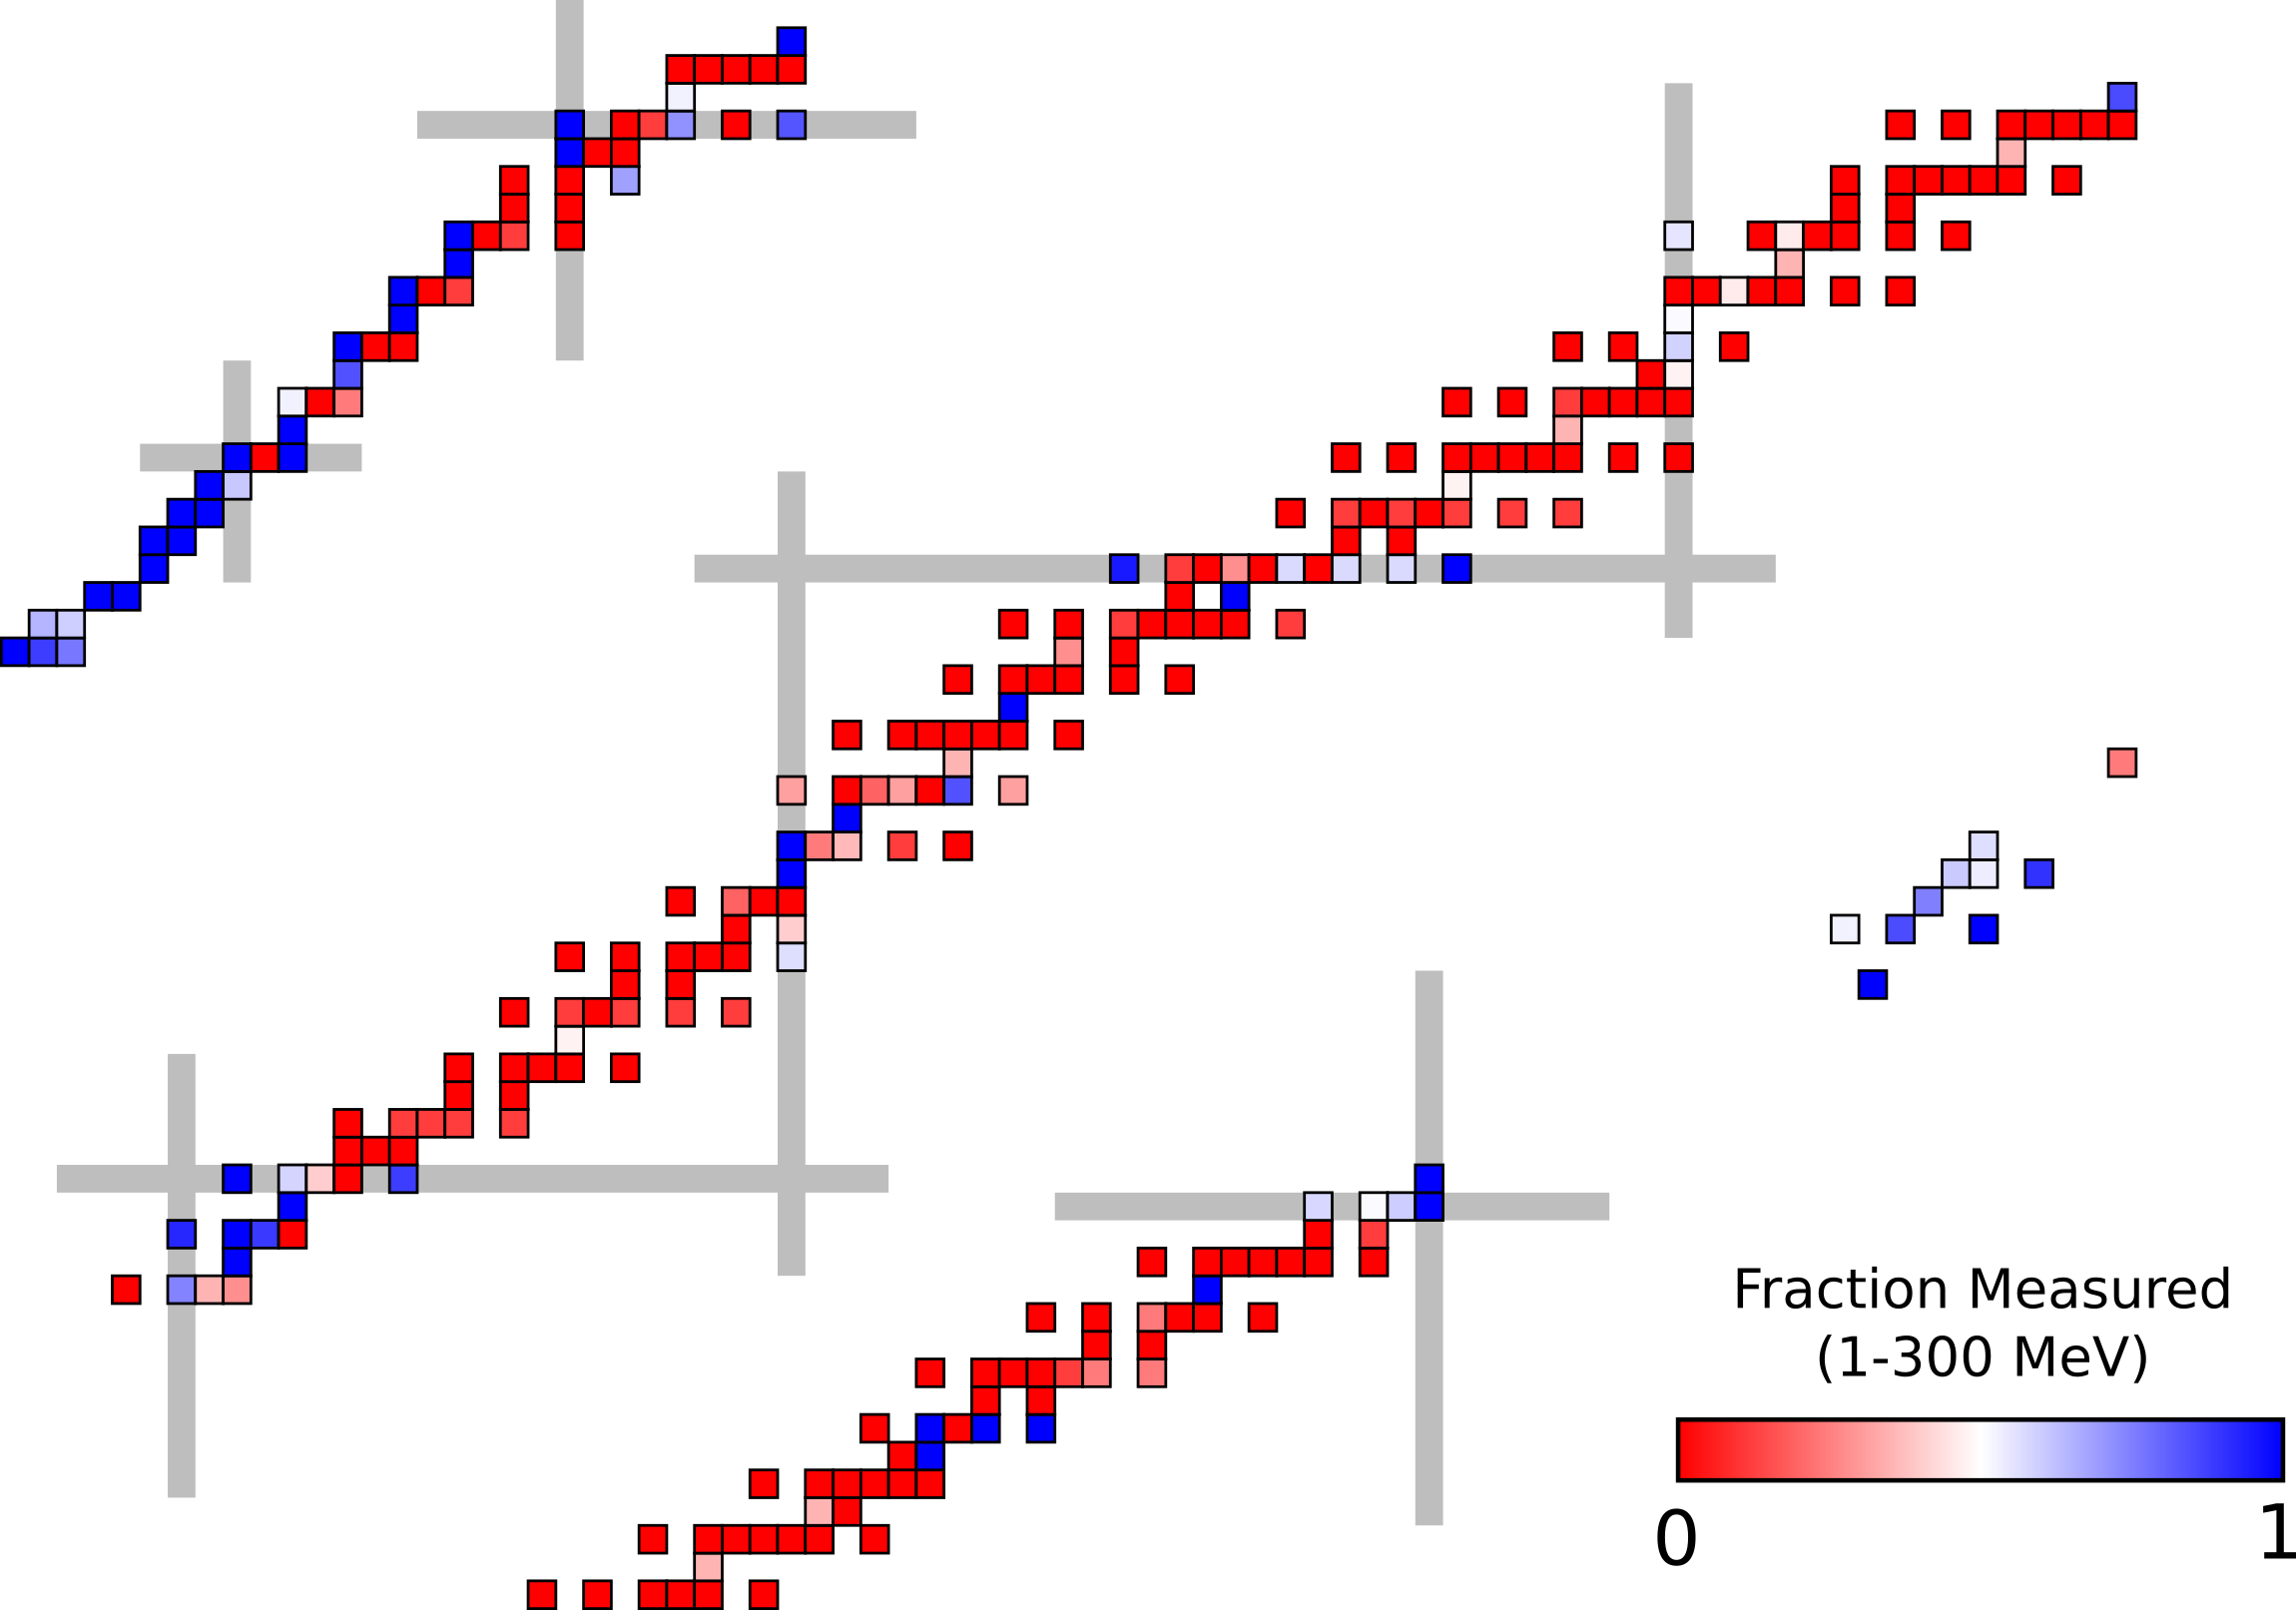
\includegraphics[width=0.8\textwidth]{figures/TCSChart.png}
    \caption{Landscape of existing neutron \tot\ data, per the EXFOR database}
    \label{TCSChart}
\end{figure}

\begin{figure}
    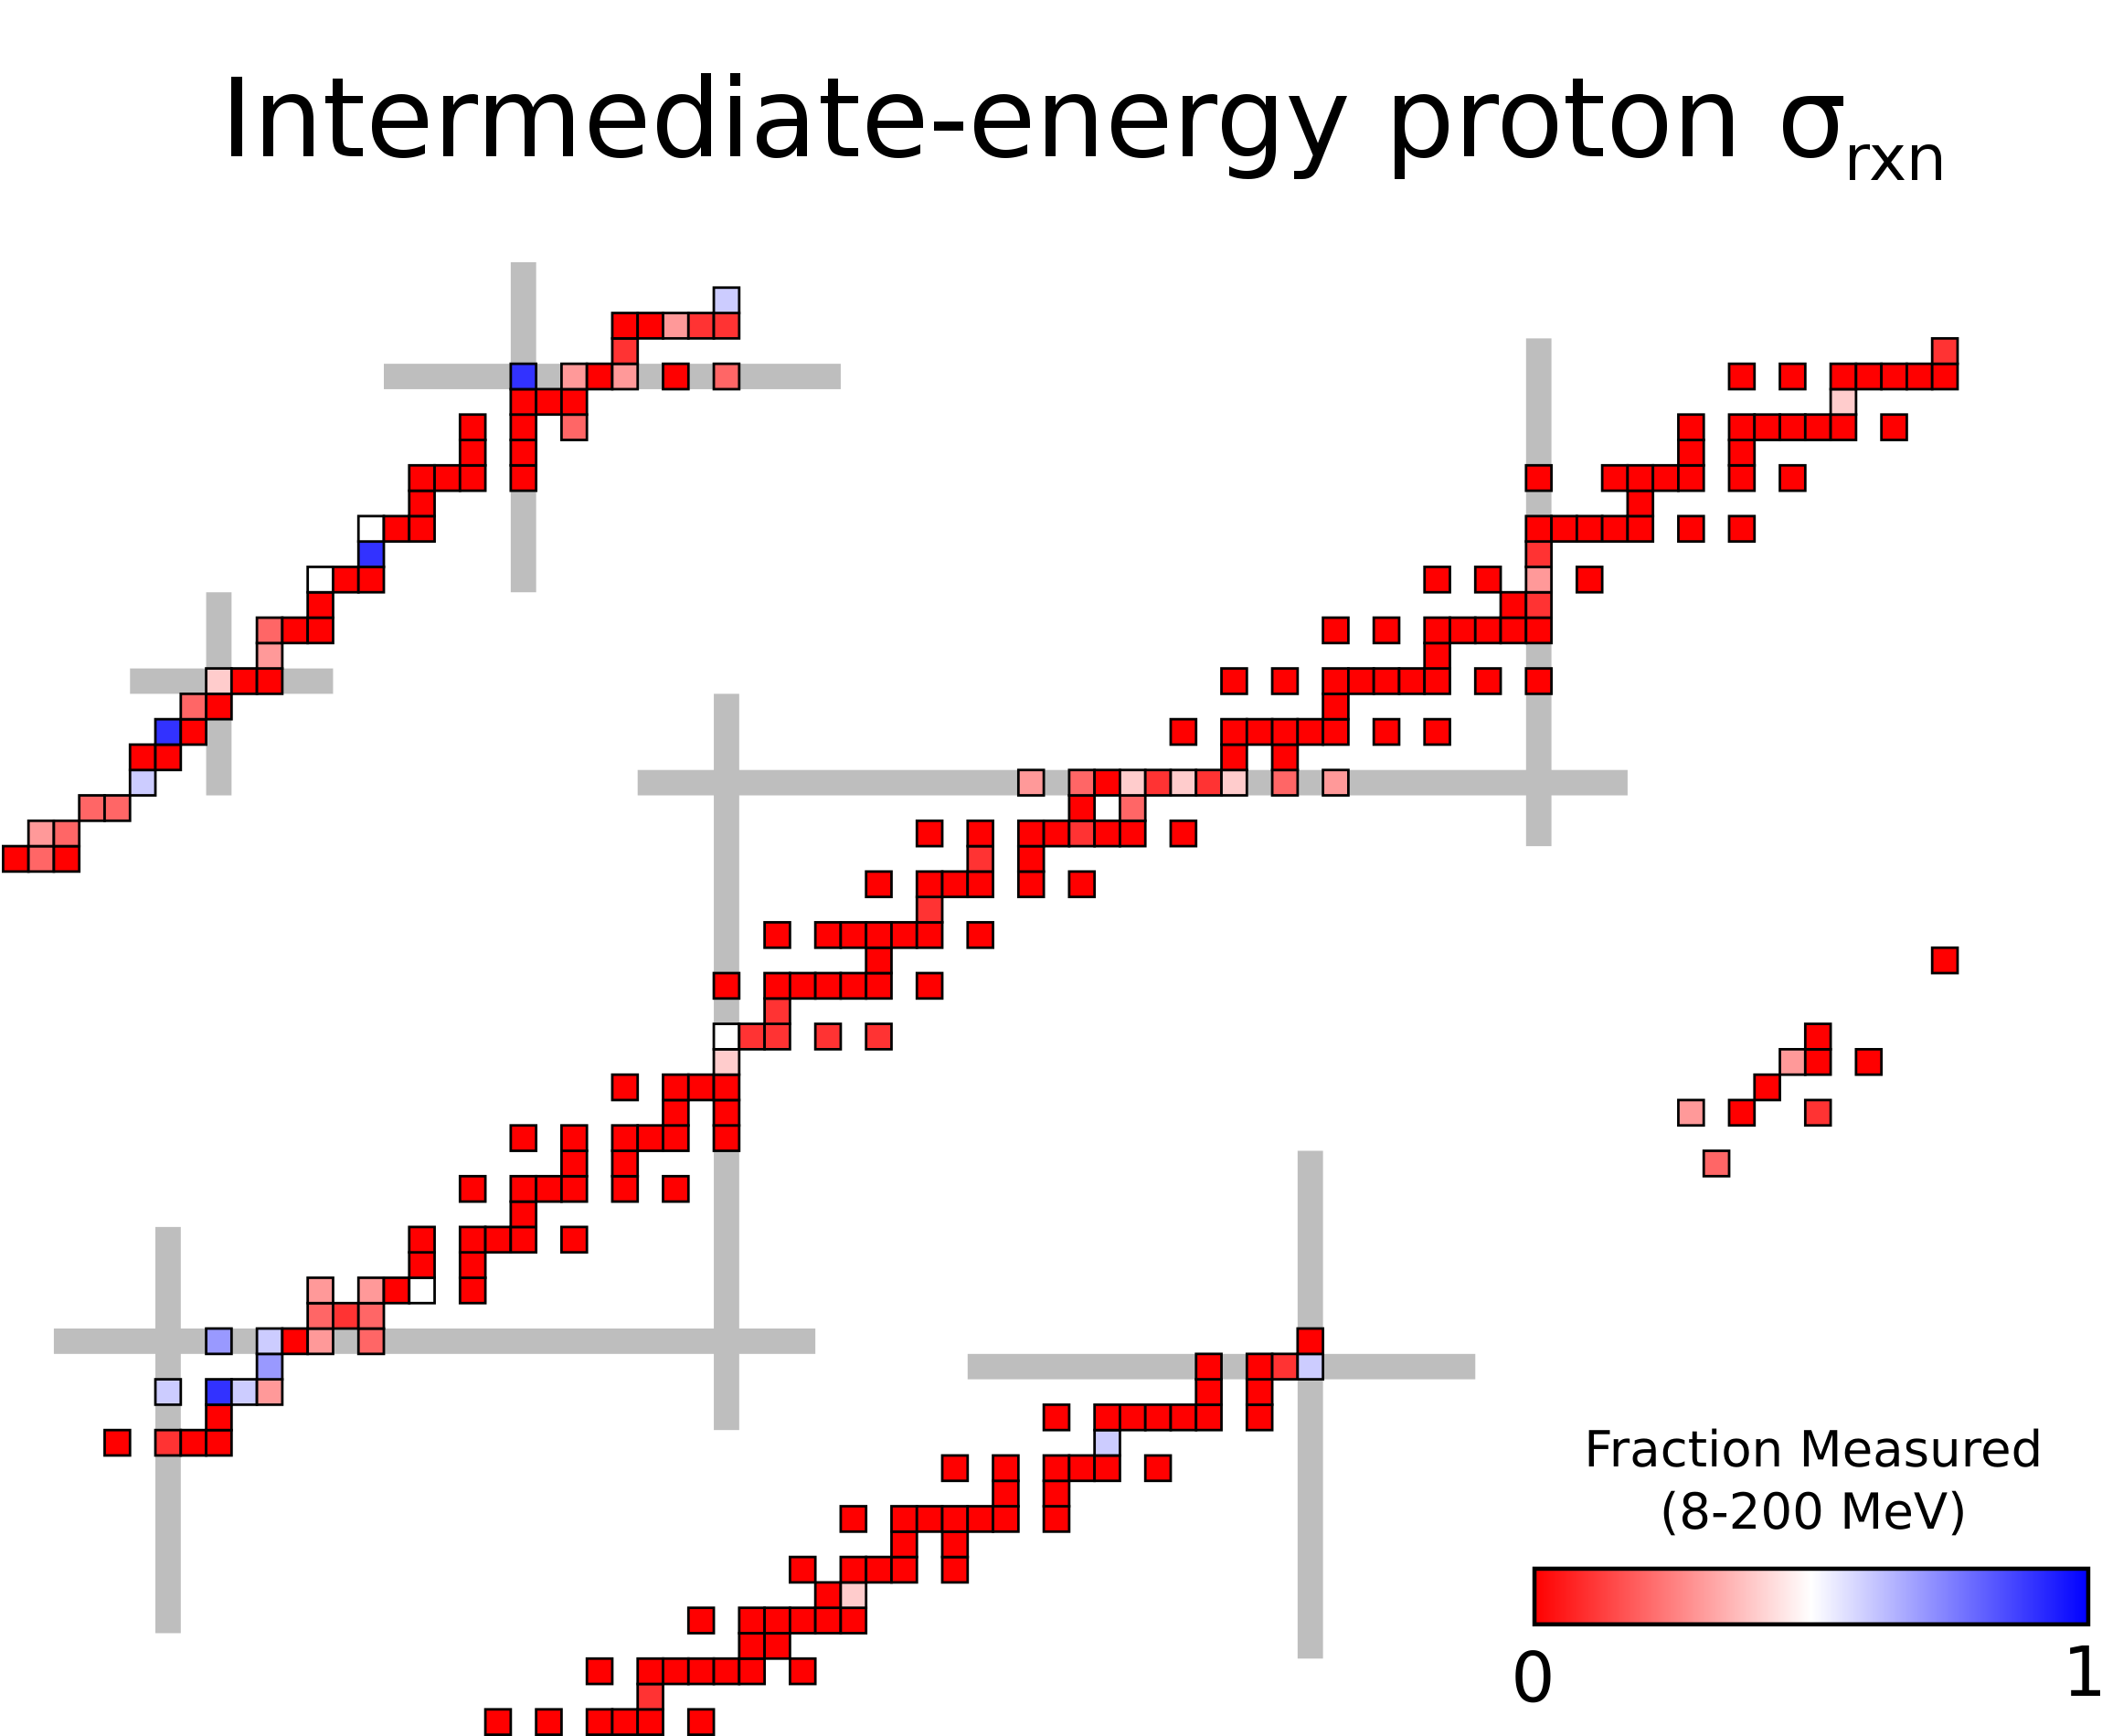
\includegraphics[width=0.8\textwidth]{figures/RCSChart.png}
    \caption{Landscape of existing proton \rxn\ data, per the EXFOR database}
    \label{RCSChart}
\end{figure}

\subsection{Electron scattering}
\subsection{Quasi-free scattering}
Louk Lapikas

\subsection{Masses and Radii}

\begin{figure}
    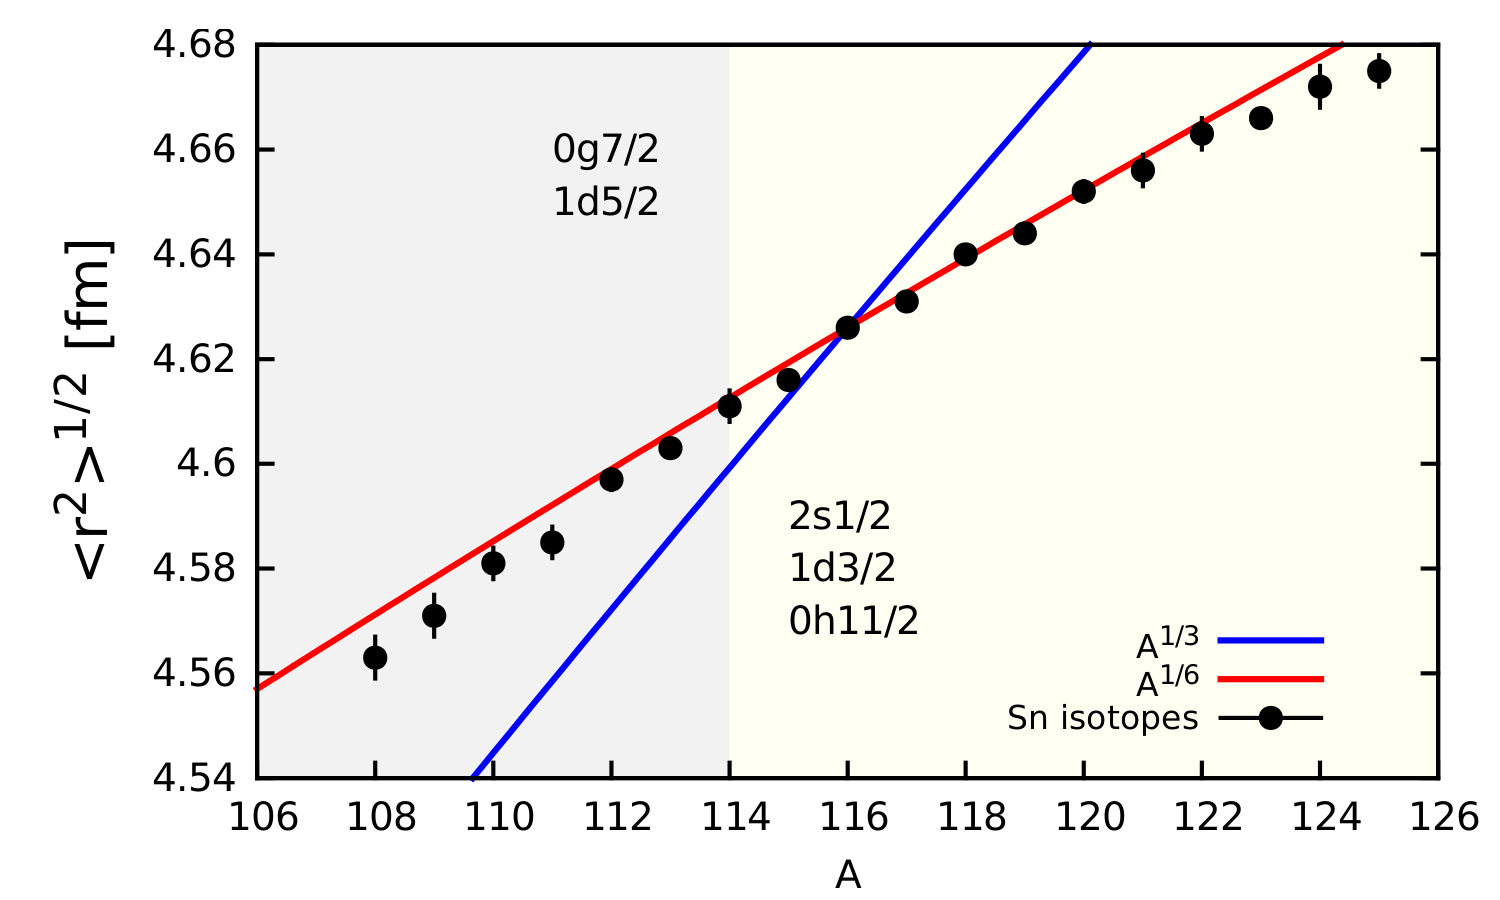
\includegraphics[width=0.8\textwidth]{figures/SnIsotopeRMSRadii.png}
    \caption{RMS charge radii in Sn nuclei, from \ref{Anselment1986}}
    \label{SnIsotopeShift}
\end{figure}

Discussion of RMS Charge Radii in Sn isotopes: Droplet model success,
Berdichevsky et al (Z. Phys. A - Atomic Nuclei 329, 393-405 (1988)) connect
slope of isotope shift to J, Q, and L of Droplet Model, Myers/Swiatecky basic
Droplet Model has L=100 and a great match to isotope shift
Isotope shift measured w/ laser spectroscopy by Anselment et al, PRC 34 p 1052,
review article by Otten (see references folder)

\section{Techniques for neutron scattering experiments}
\subsection{Neutron beam production}
Neutron production: monoenergetic (tandem, via d(d,n)3He, t(d,n)$\alpha$),
or white (reactor and spallation sources)?. Includes description of
collimation, beam production, room background issues, facilities where
available, advantages and disadvantages of each production mechanism.

\subsection{Neutron detection}
Neutron detection: fast plastic, liquid scintillators, He3 counter, CLYC array, poly
terphenyl. N-gamma discrimination by pulse shape discrimination. TOF techniques
for energy determination. Charged particle rejection. MoNA, neutron wall at
FRIB, VANDAL. Use of machine learning to distinguish gammas from neutrons.

Analog vs. digital techniques (connect to LANSCE measurements from \ref{Abfalterer2001, Finlay1993}).

At end of section, familiar with:
- neutron beam production and facilities
- a variety of neutron detection techniques: liquid/plastic scintillators,
means of energy detection and background rejection, PSD

\section{Motivation and Dissertation Overview}
With the need for improved neutron scattering data established and an overview of neutron
detection technology provided, the results of our neutron scattering measurement campaign can be
presented. The experimental layout and analysis for our isotopically-resolved \tot\ measurements are 
detailed
in Chapters \ref{TCSExperiment} and \ref{TCSAnalysis}, and for our elastic scattering measurements 
on \snTwelveFour in Chapters \ref{ECSExperiment} and \ref{ECSAnalysis}. A brief summary of the 
Dispersive Optical Model formalism is
given in Chapter \ref{DOMFormalism} in preparation for the results from our DOM fits of \oSixEight, \caAughtEight, 
\niEightFour, \snTwelveFour, and \pbEight presented in Chapter \ref{DOMResults}. Complete
details on the experimental data sets used in the analysis and figures showing the quality of the
fits are provided in Appendices \ref{DOMDataSets} and \ref{DOMFits}. 

At end of introduction:
- familiar with value of neutron scattering data for optical models and also as
fundamentally valuable for nuclear science; proton scattering data have been
accumulated, but neutron scattering data are much scarcer
- familiar with scarcity of certain types of difficult neutron and proton
scattering data (\tot, \rxnE)
- familiar with relevance to infinite nuclear matter equation of state and
neutron star radii

Questions posed:

- What do the nucleons do in the nucleus? Where are the neutrons and the protons
with respect to each other?

- What is needed to expand beyond current workhorse models (Droplet Model,
Shell Model, Optical Models) and connect nuclear reactions and structure

- What are the neutron scattering data for cornerstone nuclides (magic Z,N) and
what do they tell us about the isoscalar/isovector terms of the optical
potential and where the nucleons go/what they do in the nucleus?

- What types of experimental data are most essential for an improved understanding of nuclear
reactions and structure?

\gls{DOM}

% \Gls{DOM} for glossary term
% \noindent for no indent

%\begin{comment}
% Woods-Saxon potential 
%\end{comment}
%
%\begin{equation}
%V(r) = \dfrac{-V_0}{1+e^{(r-R)/a}},
%\end{equation}

%\mathbf{J} = math bold-font symbol 'J'
